% Setup - do not change
\documentclass[11pt]{article}
\usepackage[top=0.9in, left=0.9in, bottom=0.9in, right=0.9in]{geometry} 
\usepackage{parskip}

\usepackage[english]{babel}
\usepackage[utf8]{inputenc}
\usepackage{amsmath,amsthm,amssymb,graphicx,pdfpages,lipsum,hyperref}
\usepackage[none]{hyphenat}
\usepackage{csquotes}

\setlength\parindent{0pt}
%%%%%%%%%%%%%%%%%%%%%%%%%%%%%%%%%%%%%%%%%%%%%%%%%%%%%%%%%%%%%%%%%%%
% add other packages here if required

\usepackage[demo]{graphicx}
\usepackage{caption}
\usepackage{subcaption}
\usepackage[sorting = none]{biblatex}
\addbibresource{references.bib}

%%%%%%%%%%%%%%%%%%%%%%%%%%%%%%%%%%%%%%%%%%%%%%%%%%%%%%%%%%%%%%%%%%% the '%' symbol denotes comments

% Begin document creation
% DELETE THE \lipsum PLACEHOLDERS WHEN YOU BEGIN
\title{\textbf{Optimising Work And Profitability For Rideshare Driver's in NYC}}
\author{
Sen Turner \\
Student ID: 1168692 \\
%% Replace the link with your github repo
% 1. Remember to escape underscore (\_) in the link.
% 2. Remember to include the commit you want to submit in the link
\href{https://github.com/MAST30034-Applied-Data-Science/mast30034-project-1-senturner/tree/76afce757d46800c60b0037981d07bd6d73fd834}{Github repo with commit}
}

\begin{document}
\maketitle

\section{Introduction}

Rideshare services like Uber and Lyft have seen a rapid expansion in recent years. Advertised for their ease of entry and promise of self-employment these services are responsible for the employment of millions of American drivers (Uber alone boasting approximately 1 million drivers) \cite{uberdrivers}. Throughout this report FHV (For Hire Vehicle) and HVFHV (High Volume For Hire Vehicle) will be used to encompass all relevant rideshare services; Juno, Uber, Via and Lyft.

\subsection{Overview}

The following report will take the perspective of one of these FHV drivers within NYC (New York City), attempting to optimise their work. It is assumed that these drivers are most interested in how easy it is to get a trip and how much money they will make in a trip. Thus, we aim to predict the number of available pickups in an hour and average driver pay for these trips. To achieve this a Neural Network classification model and a Random Forest classifier will be generated using HVFHV data and weather data.  

\section{Datasets}

The taxi data has been sourced from the TLC Trip Record Data \cite{taxidata}. Due to the inherent focus of this report on rideshare service drivers, the High Volume For Hire Vehicle taxi type has been isolated. This dataset includes relevant information including date, time and location of pickup as well as driver pay amount, which directly represent or potentially impact driver's profitability.

To supplement the taxi data, NYC weather data has been source from WUnderground \cite{weatherdata}. The Jackson Heights weather station was used as a summary of overall NYC weather, as significant deviations across NYC were assumed unlikely. This dataset includes weather factors such as temperature, precipitation rate, wind speed, air pressure and humidity, which logically are expected to correlate with rideshare demand. 

\subsection{Attribute Decisions}

The chosen attributes are such that a FHV driver could know them in advance, allowing them to make optimal decisions about when and where to drive. For this reason, features such as trip time was not included, because this information is unavailable to drivers before the ride.

\subsection{Timeline}

A timeline starting from first availability of HVFHV (start of February 2019) was used. Due to COVID-19 New York City went into lockdown in March of 2020, clearly impacting the demand for rideshare services as seen in Figure 1. However, presence of weather data in the study requires at least a one year timeline in order to account for seasonal effects. Thus to avoid any impact of COVID-19 data, but maintain at least a year long timeline, data was used until start of February 2020.

\begin{figure}[h]
    % change the scale multiplier to make the figures smaller or larger
    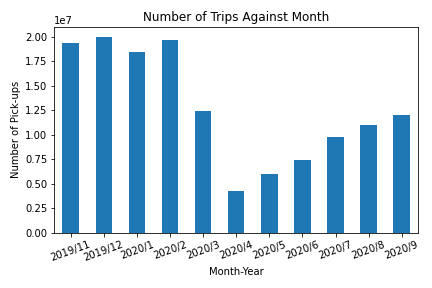
\includegraphics[width=0.6\textwidth]{plots/trips_v_month.png}
    % this ensures your figures are centered where possible
    \centering
    \caption{Number of FHV Trips between 2019/11 and 2020/9 (incl.)}
\end{figure}

\section{Pre-processing}

The format of both datasets is relatively consistent, there are of course outliers that exist outside of the expected framework. The pre-processing section focuses on how we deal with such instances.

The overall pre-processing pipeline involved:
\begin{enumerate} 
    \item Removing invalid records
    \item Feature selection
    \item Format/type conversions (for dataset combination)
    \item Outlier detection/Imputation
    \item Aggregation
\end{enumerate}

\subsection{Feature Selection}

A Pearson correlation matrix, seen in Figure 2, was formed for the weather data in an attempt to reduce the number of features. This saw the removal of dew point, wind gust and precipitation accumulation because they were heavily correlated with other, more outwardly informative, features. Similarly, features that were unlikely to influence FHV demand, like solar irradiance, were removed.

\begin{figure}[h]
    % change the scale multiplier to make the figures smaller or larger
    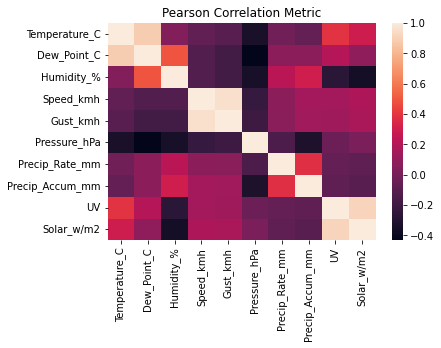
\includegraphics[width=0.6\textwidth]{plots/weather_correlation.png}
    % this ensures your figures are centered where possible
    \centering
    \caption{Pearson Correlation Matrix of Weather Features}
\end{figure}

In the FHV data, features that a driver could not control in advance or seemed irrelevant to the study goal were removed. For example, pick-up location was retained but drop-off location was not (driver can control where they wait for trips, but not where the trips go). Additionally, new features that were expected to be highly correlated with demand, like day of the week and hour of the day, were extracted from the datetime feature.

After selection, the following features were used for analysis and model fitting.

From the weather dataset: Date and Time, Temperature, Wind speed, Humidity, Precipitation Rate and Pressure.

From the taxi dataset: Pick-up Date and Time, Pick-up Location ID, Driver pay, Day of Week, Hour of Day.

It must be noted that exact date and time were not used for the eventual model fitting because this would lead to significant over-fitting.

\subsection{Outlier Detection}

224,634,939 instances remained after removal of invalid records and combination of downloaded datasets. Further detection was required to remove the following types of outliers.

Trips with dates outside of desired range, saw the removal of roughly 750,000 records due to extra downloads.

Trips over 4 hours in length. These trips made up a very small minority of rides, only 7649, but have significantly large driver pay due to their length. Thus, they were removed following the conclusion that drivers could not reasonably rely on these long trips, meaning models would more accurately reflect day-to-day reality without them.

Trip's with pick-up IDs outside of the desire 1-263 range. There were only 12918 instances of such trips.

\subsection{Imputation}

Following the previous steps imputation was not required. Weather data was available for all the hours of the year, meaning all FHV records had relevant weather data. Similarly, no FHV records were missing the relevant information.

\subsection{Aggregation}

The aim of this report is to model and thus optimise the number of trips in an hour and the average driver pay for these trips. Thus, it is not important to maintain information about individual trips and model can be trained on aggregated statistics.

The aggregation step was performed by grouping the data over date, hour and pick-up location id, then averaging the driver fare for all these trips and counting the total number of trips.

Some different aggregations (including over just date and hour), were used for visualisation in order to reduce clutter.

\section{Analysis}

This section is responsible for investigation of the relationships between features and target variables (number of trips and average driver fare).

\subsection{Pickup Location}

\subsubsection{Number of Trips}

This feature is clearly correlated with the number of trips. Figure 3 demonstrates that the number of trips taken from different locations are vastly different. Locations in central Manhattan and at JFK and LaGuardia airports have millions more trips than the less popular outer suburbs in the year long period.

\begin{figure}[h]
    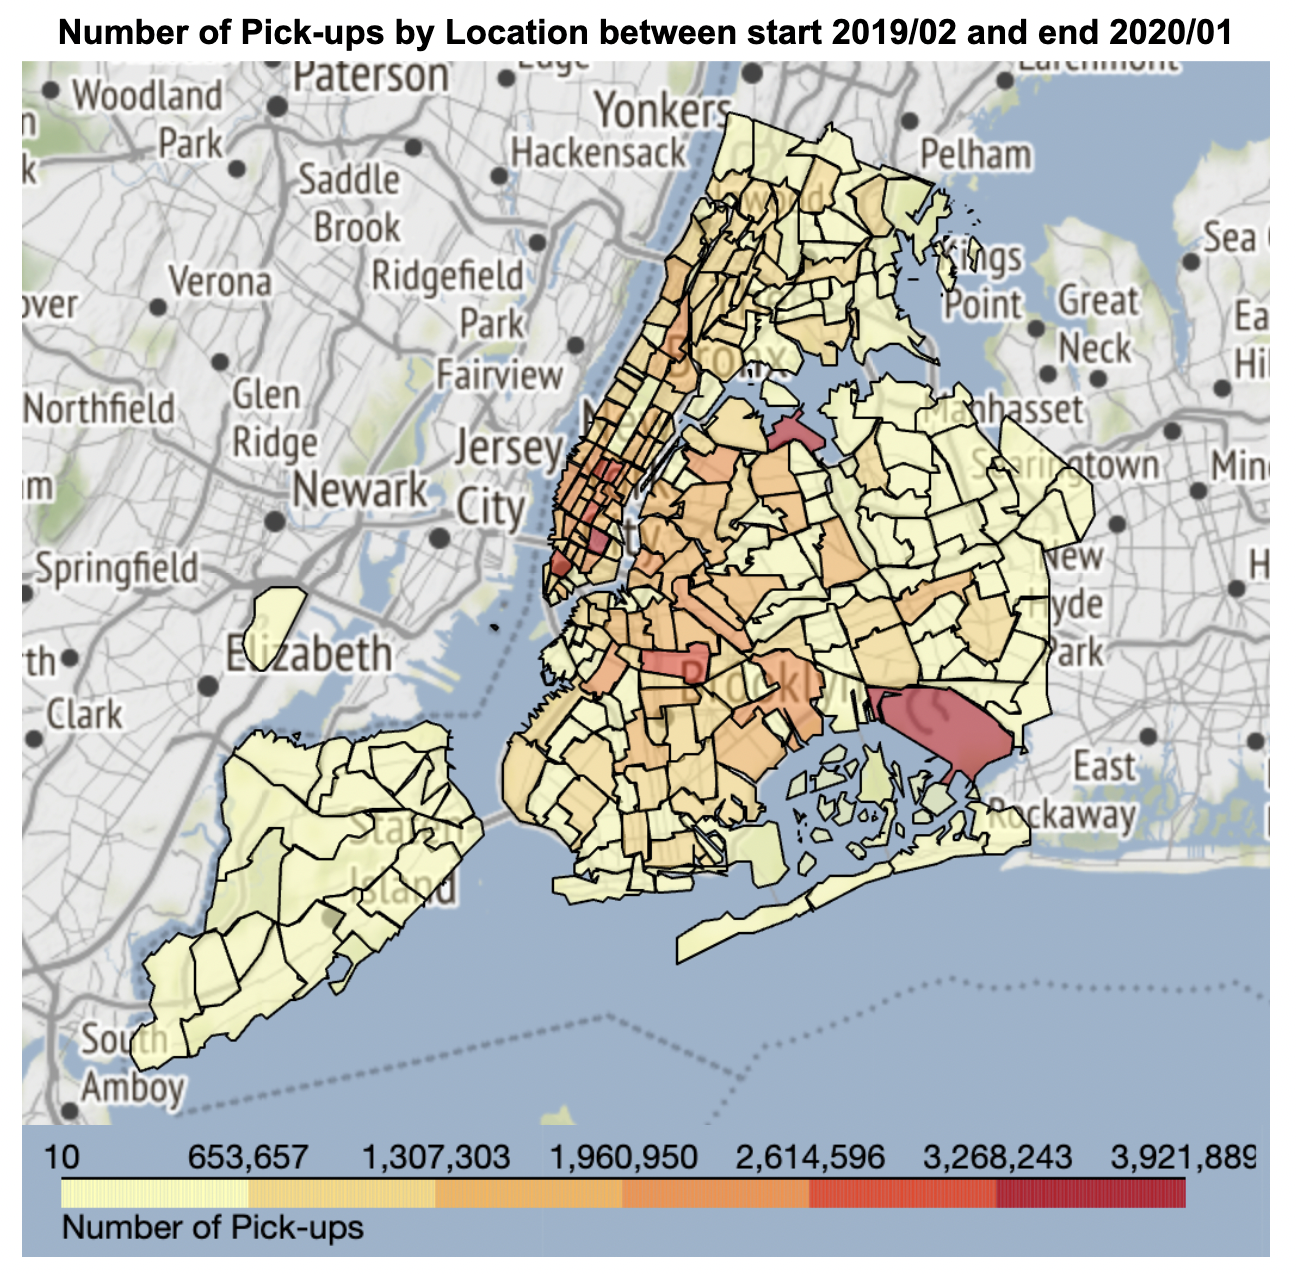
\includegraphics[width=0.5\textwidth]{plots/num_trips_map.png}
    \centering
    \caption{Number of Trips (Pick-ups) by Location Between 2019/02 and 2020/01 (incl.)}
\end{figure}

\subsubsection{Average Driver Pay}

Pickup location is also clearly correlated with number of trips. Figure 4(a) reflects this fact, particularly for airports, which have average prices \$20-\$30 higher than less expensive areas. This is intuitive because people at airports are more likely to travel further, meaning higher pay.

This motivates further analysis of average pay outside of the airports, seen in Figure 4(b). Similarly to number of trips, central Manhattan has higher prices, along with areas around LaGuardia and JFK airports.

\begin{figure}[h]
\centering
\begin{subfigure}{.5\textwidth}
  \centering
  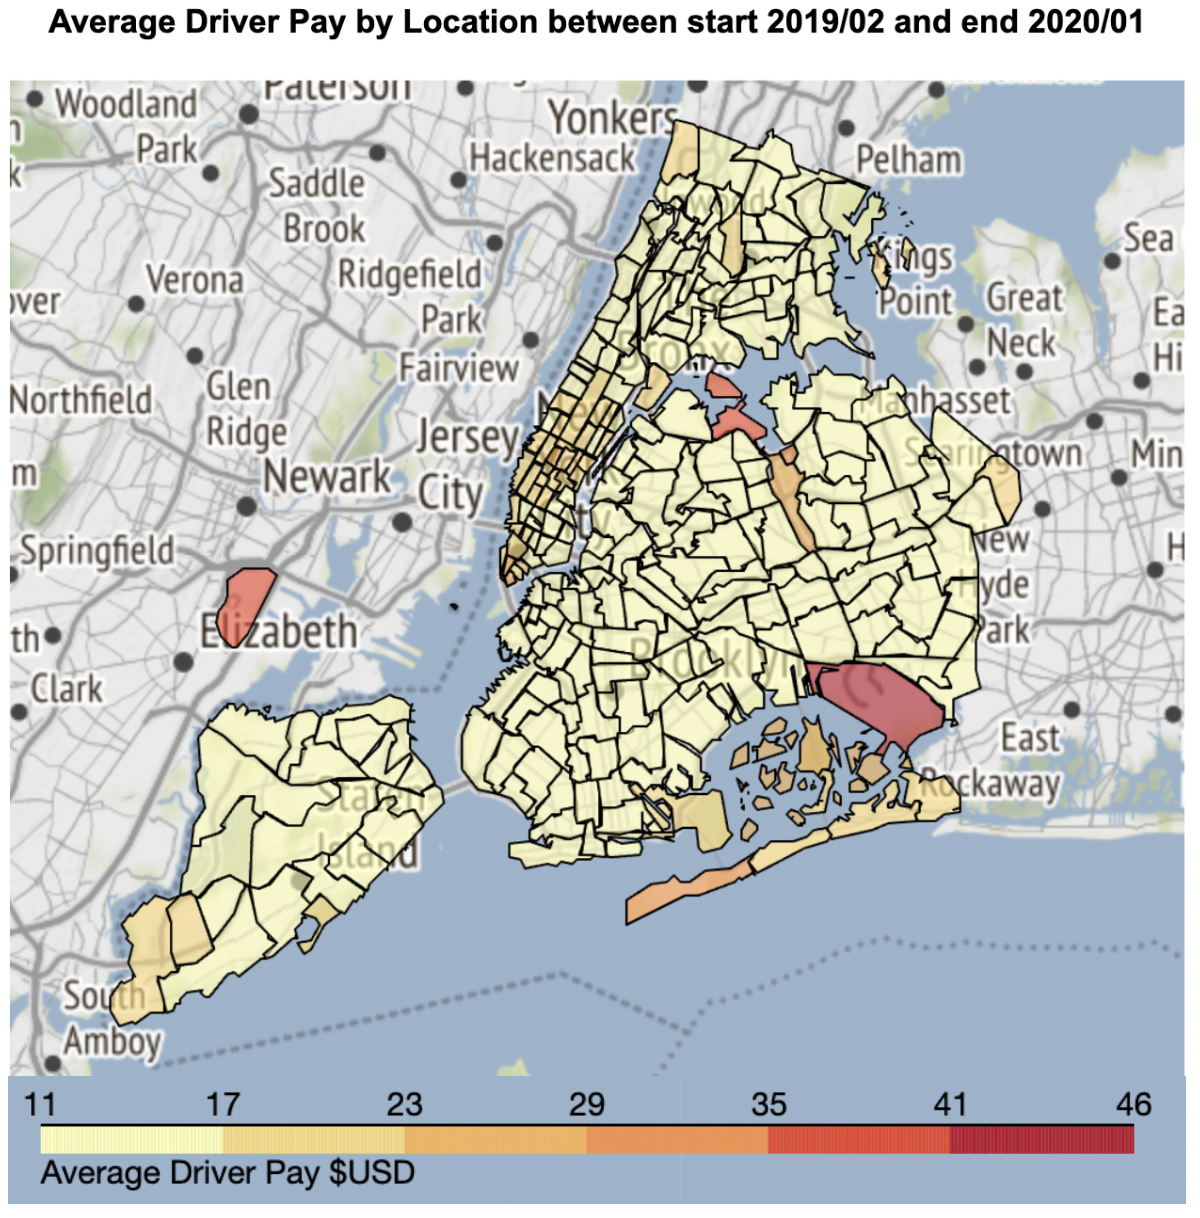
\includegraphics[width=1\linewidth]{plots/avg_pay_map.png}
  \caption{Airports Included}
  \label{fig:sub1}
\end{subfigure}%
\begin{subfigure}{.5\textwidth}
  \centering
  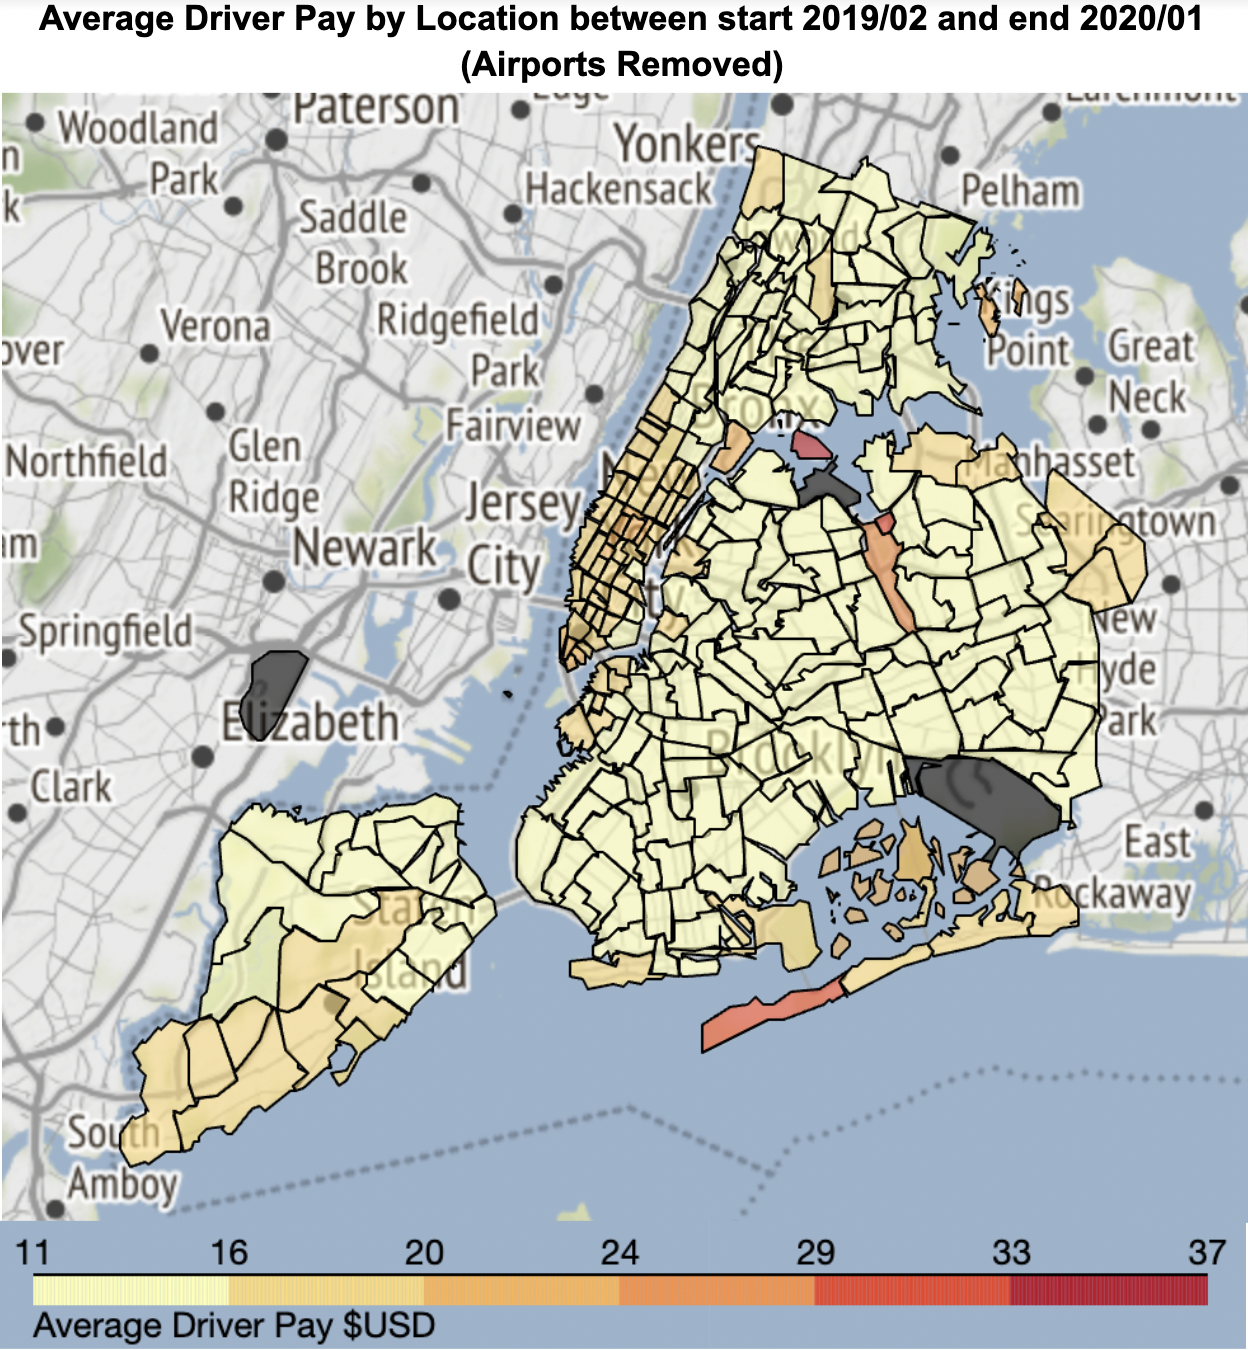
\includegraphics[width=1\linewidth]{plots/avg_pay_map_air.png}
  \caption{Airports Removed}
  \label{fig:sub2}
\end{subfigure}
\caption{Average Driver Pay \$USD by Location}
\label{fig:test}
\end{figure}

\subsection{Hour of Day and Day of Week}

Visualisations for these features were produced using a sample of the dataset corresponding to 1200 hours of data in order to improve clarity.

\subsubsection{Number of Trips}

Figure 5(a) demonstrates the relationship between day of the week and number of trips. There is a slight increase in the number of trips over the weekend, particularly Friday and Saturday, which was intuitively expected. Figure 5(b) conveys the correlation between hour of the day and number of trips, as trip counts clearly vary across the different hours. The increased number of trips between 7-9am can possibly be attributed to travel to work. Similarly, the increase towards the end of the day is potentially explained by travel to bars/restaurants.

\begin{figure}[h]
\centering
\begin{subfigure}{.5\textwidth}
  \centering
  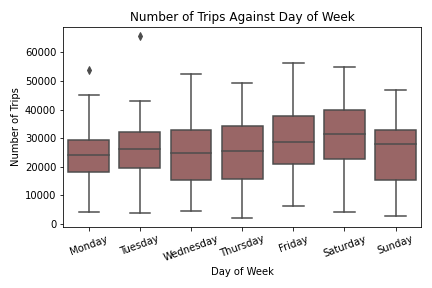
\includegraphics[width=0.9\linewidth]{plots/trips_v_day.png}
  \caption{Number of Trips Against Day of Week}
  \label{fig:sub1}
\end{subfigure}%
\begin{subfigure}{.5\textwidth}
  \centering
  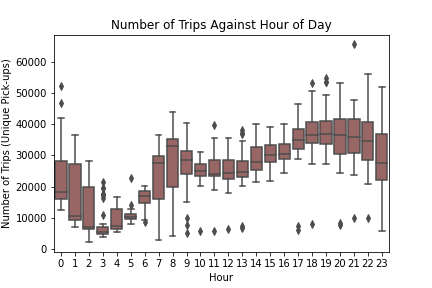
\includegraphics[width=0.9\linewidth]{plots/trips_v_hour.png}
  \caption{Number of Trips Against Hour of Day}
  \label{fig:sub2}
\end{subfigure}
\caption{Number of Trips at Different Time}
\label{fig:test}
\end{figure}

\subsubsection{Average Driver Pay}

The relationship between time and average driver pay is also made evident in Figures 6(a) and 6(b). However, the results are less intuitive than number of trips. Average pay appears to increase during hours and days when demand is low, with high average pay in the early hours and lower average pay on Saturday and Sunday. This is potentially due to FHV features like `surge' pricing \cite{surge}.

\begin{figure}[h]
\centering
\begin{subfigure}{.5\textwidth}
  \centering
  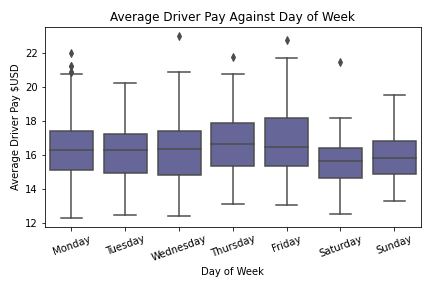
\includegraphics[width=0.9\linewidth]{plots/pay_v_day.png}
  \caption{Average Driver Pay Against Day of Week}
  \label{fig:sub1}
\end{subfigure}%
\begin{subfigure}{.5\textwidth}
  \centering
  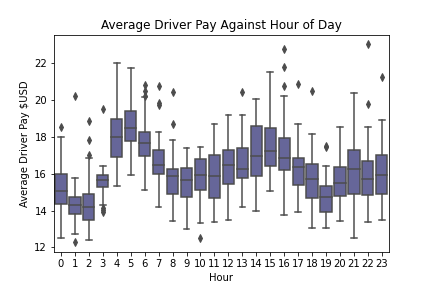
\includegraphics[width=0.9\linewidth]{plots/pay_v_hour.png}
  \caption{Average Driver Pay Against Hour of Day}
  \label{fig:sub2}
\end{subfigure}
\caption{Average Driver Pay at Different Time}
\label{fig:test}
\end{figure}

\subsection{Weather}

To explore relationship between target variables and weather data, ANCOVA was performed using hour of day as a covariate variable. Hour of day was chosen because it was expected to correlate heavily with weather conditions, thus requiring removal of the variance caused by this confounding feature.
 
\begin{minipage}[c]{0.45\textwidth}
\resizebox{1\textwidth}{!}{
\begin{tabular}{||c c c c c||} 
 \hline
 Source & SS & df & F & Pr(\ge F) \\
 \hline
 Hour & 2.53e+09 & 23 & 8941.7 & 0 \\ 
 \hline
 Temperature & 5.22e+07 & 1 & 4243.5 & 0.0 \\
 \hline
 Wind Speed & 2.60e+06 & 1 & 211.6 & 6.07e-48 \\
 \hline
 Humidity & 8.38e+05 & 1 & 68.1 & 1.54e-16 \\
 \hline
 Precip Rate & 1.70e+07 & 1 & 1386.4 & 2.38e-303\\ 
 \hline
 Pressure & 3.64e+04 & 1 & 2.96 & 0.085\\
 \hline
 Residual & 2.68e+10 & 2177375 & & \\  [1ex]
\end{tabular}
}
\captionof{table}{ANCOVA Table For Weather Predictors and Number of Trips}
\end{minipage}%
\hspace{0.05\textwidth}
\begin{minipage}[c]{0.45\textwidth}
\resizebox{1\textwidth}{!}{
\begin{tabular}{||c c c c c||} 
 \hline
 Source & SS & df & F & Pr(\ge F) \\
 \hline
 Hour & 3.45e+06 & 23 & 5332.9 & 0 \\ 
 \hline
 Temperature & 2.49e+05 & 1 & 8835.9 & 0.0 \\
 \hline
 Wind Speed & 1.18e+04 & 1 & 420.7 & 1.77e-93	 \\
 \hline
 Humidity & 1.89e+03 & 1 & 67.3 & 2.28e-16 \\
 \hline
 Precip Rate & 5.50e+03 & 1 & 195.6 & 1.93e-44 \\ 
 \hline
 Pressure & 5.59e+02 & 1 & 19.9 & 8.31e-06 \\
 \hline
 Residual & 6.13e+07 & 2177375 & & \\  [1ex]
\end{tabular}
}
\captionof{table}{ANCOVA Table For Weather Predictors and Average Driver Pay}
\end{minipage}

Table 1 and Table 2 demonstrate clear correlation between temperature, humidity, wind speed, precipitation rate and both number of trips and average driver pay, reflected by significantly low p-values. However, pressure has a p-value of 0.085 with number of trips. This indicates the impact of this feature is not particularly significant, leading to the decision (though not absolutely necessary) to exclude pressure from eventual model training.

\section{Models}

To model the hourly average driver pay and number of trips neural network and random forest classifier have been chosen. These models are chosen due to their high performance and suitability for large datasets. The models can also capture non-linear relationships between features and target variables, which may be important for weather features like temperature. Additionally, correlation between variables like weather and hour will not cause issues in either model.

It must be noted that predictions and testing were required to be performed on future data, limiting testing to the last 20\% of the dataset. This means only data from the the end of the year (Winter/cold climate) was used for testing, while training was performed on warmer months.

\subsection{Neural Network}

Individual neural network models were trained for both average driver pay and number of trips. Categorical variables were one-hot encoded and values were normalised so that features with large magnitude are not prioritised by the network.

Through testing, a shallow network architecture was seen to have higher performance. This lead to using a single, fully connected hidden layer with 10 neurons for both networks. The average pay model took 5 epochs for validation loss to converge, while number of trips model took 10 epochs to stabilise. 

Mean square error was used to measure the loss of both networks. Testing performance gave mean square error of 11.05 for average pay model and 2199.35 for number of trips. This lead to r-squared statistics of 0.4489 and 0.8155 respectively.

\subsection{Random Forest}

Individual random forest models were trained for both average driver pay and number of trips. Random forest can handle numeric and categorical data inherently so no transformation was required. 

270 max bins was required due to the large number of pick up locations. Max depth of 5 was used to avoid over-fitting and 20 trees were used to maintain model efficiency. 

Testing model performance gave mean square error of 13.67 for average pay model and 3502.34 for number of trips. This lead to r-squared statistics of 0.4401 and 0.7062 respectively.

\subsection{Model Comparison}

The neural network model had lower mean square error during testing for both average fare and number trips. However, this metric is not that useful in isolation. 

Figure 7 compares ground truth against model predictions for the 30th November 2019 in Allerton/Pelham Gardens, though results are similar for different dates and locations.

\begin{figure}[h]
\centering
\begin{subfigure}{.5\textwidth}
  \centering
  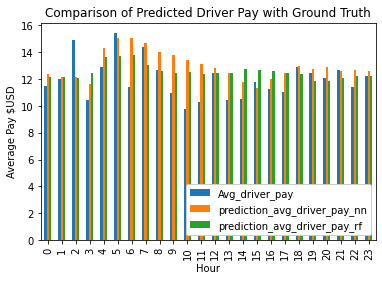
\includegraphics[width=0.9\linewidth]{plots/hourly_pay_predictions.png}
  \caption{Average Driver Pay Predictions vs Ground Truth}
  \label{fig:sub1}
\end{subfigure}%
\begin{subfigure}{.5\textwidth}
  \centering
  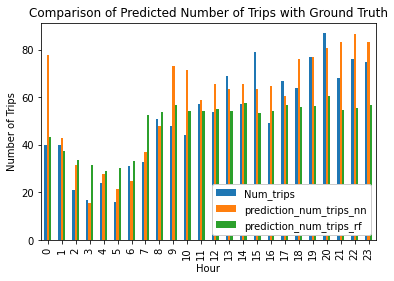
\includegraphics[width=0.9\linewidth]{plots/hourly_trips_predictions.png}
  \caption{Number of Trips Predictions vs Ground Truth}
  \label{fig:sub2}
\end{subfigure}
\caption{Model Predictions Against Ground Truth}
\label{fig:test}
\end{figure}

Both models perform quite well at predicting number of trips and average fare. It is evident that the random forest is more conservative in its predictions, as the predicted number of trips doesn't vary significantly outside of early hours in the morning. Contrasting this, the neural network appears more bold, leading to occasional significantly incorrect predictions, but better mapping of the overall trends in number of hourly trips.

The predictions made by both models support the idea that FHV drivers should target later hours due to the increased number of trips, making it easier to find jobs. Similarly, the models' predictions indicate that they captured information surrounding higher average driver pay in early hours. Solidifying early analysis which suggested this may be the case.

\section{Recommendations and Conclusions}

The relative success of the models means it is entirely plausible that a FHV driver could use a model to predict and thus optimise their average pay and number of trips, maximising their profitability.

Thus, the report ideally suggests that FHV drivers gain access to a neural network or random forest model to predict the number of available trips and their average pay. This could be achieved through individually producing a model or by FHV companies like Uber adding this functionality to their apps to improve driver experience. Thus, drivers could use the models to choose the conditions that they will work under in order to maximise their profits. For example, drivers can choose the day and hour, target location and weather conditions based on number of trips, average pay or both. 

Additionally, visual analysis suggested that drivers should prioritise working around the JFK and LaGuardia airports due to the high number of trips and high average pay for these trips. Central Manhattan was also a stand-out location for these metrics. Similarly, number of trips increased over the weekend and in the late hours of the day, implying drivers should target these times if they want consistent trips. However, the higher average pay in early hours also implies towards driver potential to target  features like surge pricing in order to maximise their pay per trip.

The findings of this report could be expanded upon by increasing the scope. It is recommended that any further advancements incorporate additional potentially impactful features. Some potential examples are effect of public events (sports games/concerts), availability of public transport and traffic. The focus area of this study could also be expanded beyond New York City to see if trends are consistent in different locations.

\clearpage

% BEGIN REFERENCES SECTION
\printbibliography

\end{document}